\section{\icecube{}}
The \icecubeneutrinoobservatory{} is a neutrino telescope
  located close to the geographic South Pole
  in proximity to the Amundsen-Scott South Pole Station.
% █ Why the South Pole?
It utilizes the optically clear Antarctic ice as detector material,
  with a total detector volume of \SI{1}{\cubic\kilo\meter} \cite{icecube_aartsen}.
The detector is composed of \num{86} strings,
  each consisting of \num{60} digital optical modules (\textsc{Dom}s),
    which are positioned
      \SI{17}{\meter} apart along the string
      at depths ranging from \SI{1450}{\meter} to \SI{2450}{\meter} below the surface \cite{icecube_aartsen}.
Each of the \num{5160} \textsc{Dom}s is equipped with a sensitive photomultiplier tube (\textsc{Pmt}),
  which is used to detect the Cherenkov light emitted by charged particles
  that interact with the ice.
%
\autoref{fig:img:icecube} shows a schematic of the \icecube{} detector.

% \icecube{} detects 275 atmospheric neutrinos daily and about 100,000 per year.


\begin{figure}
  \centering
  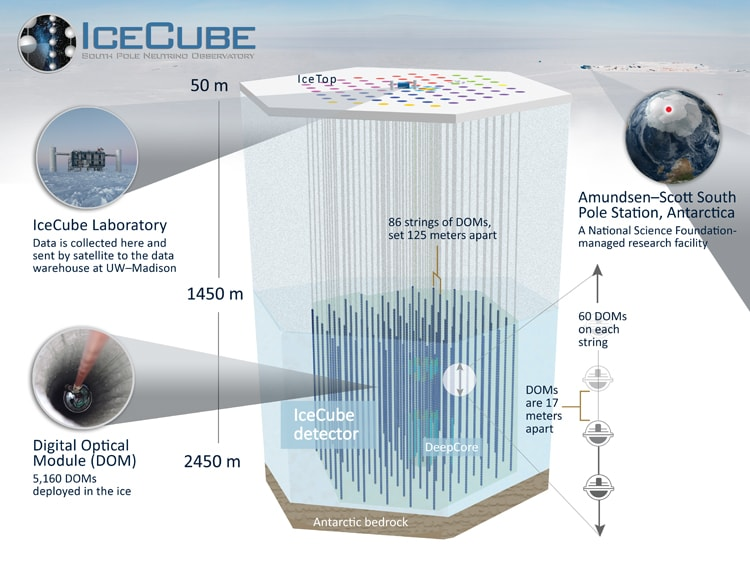
\includegraphics[width=0.8\textwidth]{content/img/icecube_detector_schematic.jpg}
  \caption{
    % Schematic representation
    % Overview
    Infographic
    of the \icecubeneutrinoobservatory{} \cite{icecube_homepage}.
    Each dot represents a \textsc{Dom}.
    % TODO: longer description
  }
  \label{fig:img:icecube}
\end{figure}


% \subsection{Detection Principle}

% █ Interaction with matter
Neutrinos interact with matter via the weak interaction.
In order to compensate for the low cross-section of the weak interaction,
  the effective detector volume is maximized by utilizing existing naturally occurring detector materials,
  such as
    the Earth's atmosphere,
    the sea,
    or the ice in the Antarctica.

When a neutrino interacts with a nucleus in the ice,
it produces a charged lepton and a neutrino.
The charged lepton then produces a Cherenkov light cone
  as it propagates through the ice
    with greater speed than the speed of light in the ice.
The light is detected by the \textsc{Pmt}s
  and the direction of the neutrino can be reconstructed
    from the position of the \textsc{Dom}s
      that detected the light.
The intensity of the light and the number of \textsc{Pmt}s that detected it
  can be used to determine the energy of the neutrino.

%     - Flavor-dependent shapes
%       - e: cascade
%       - µ: track
%       - ν: double bang / lollipop

% ↓ https://journals.aps.org/prd/abstract/10.1103/PhysRevD.68.093005
% █ showers (νe charged current, most ντ charged current, and all flavors neutral current)
% █ muon tracks (νμ charged current only)
% █ tau lepton lollipops and double bangs (ντ charged current only)

Depending on the flavor of the leptons,
  different types of interactions occur,
  which can be used to determine the flavor of the neutrino.
% ↓ TODO Copilot!
Electron neutrinos ($\nu_e$) and muon neutrinos ($\nu_\mu$) are produced by the weak interaction,
  while tau neutrinos ($\nu_\tau$) are produced by the weak interaction
  and the tau lepton decay.
Examples of interactions and detector patterns are shown in \autoref{fig:img:icecube:interactions}.

\phantomsection \label{sec:neutrino_astronomy:icecube:up_going}
Not only neutrinos leave can leave traces in the detector, % interact with the ice,
  but also atmospheric muons.
For this reason,
  the detection is mostly limited to \emph{up-going} events \cite{icecube_aartsen},
  % ($\SI{0}{\degree} < \theta < \SI{180}{\degree}$)
  % ORIG: Up-going events for all triggered energies are selected, while only high-energy down-going tracks are selected to avoid the large background of down-going atmospheric muons at lower energies.
    because muons
      – in contrast to neutrinos –
    are mostly blocked by the Earth's mass.

%   - Triggering / reconstruction / feature extraction
% █ Numbers and facts
% █ Achievements


